%!TEX root = Tesi__Simone_Mariotti.tex
\chapter{Visione Artificiale}
\fancyhead[R]{\bfseries Visione Artificiale} 	 	
\fancyfoot[C]{\thepage } 
La \textit{visione artificiale} è l'unione dei procedimenti che permettono di 
creare  un modello del mondo reale in tre dimensioni a partire da numerose 
immagini bidimensionali per cercare di emulare il processo biologico della vista.
Negli umani, così come in molte altre specie, vedere non è solo scattare una 
fotografia bidimensionale mentale di un ambiente, è interpretare le informazioni
ricevute attraverso la retina per analizzare e creare un modello 3D dell'ambiente
 circostante.\\	
Un sistema di visione artificiale, per provare ad avvicinarsi alla capacità visiva
e di interpretazione umana, ha bisogno di numerosi componenti di diversa natura: 
ottici, elettronici e meccanici per acquisire e memorizzare le immagini da elaborare.
Il primo tentativo in tal senso è datato 1883 quando  Paul Gottlieb Nipkow 
inventò il primo sistema 
in grado di traformare o meglio trasdurre, informazioni visive in un segnale elettrico. Il sistema
 si basa su un disco con dei fori equidistanti e di egual raggio lungo una 
 spirale che gira ad una velocità costante, l'immagine inquadrata viene indirizzata 
 verso i fori da una lente, un sensore sul retro del disco trasforma le variazione 
 di luminosità in segnali elettrici. Il ricevutore emetterà luce in base ad i 
 segnali elettrici e attraverso un disco identico al primo e in rotazione sincrona 
 proietterà un'immagina con tante righe quante sono i fori del disco.
 Questo sistema porterà alla creazione della TV meccanica nel 1925.
 \begin{figure}[!htb] \center
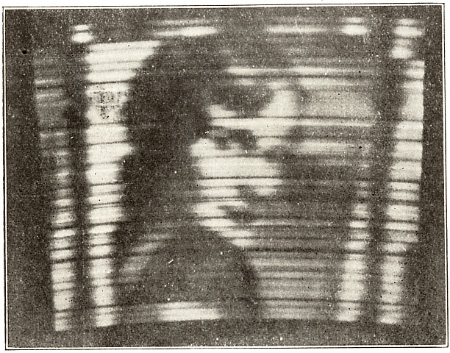
\includegraphics[width=\textwidth]{immagini/tv_meccanica.png}
\caption{Immagine visibile su una TV meccanica del 1925} 
\end{figure}
\\Da quel periodo si sono fatti enormi progressi grazie alla miniaturizzazione 
dell'elettronica. Gli scienziati per produrre un effetto sempre migliori si sono
ispirati alla macchina migliore che esiste, il corpo umano: analizzando da vicino
l'occhio e in particolare la retina si sono resi conto che era formata da minuscoli 
recettori sensisbili alla luce, ognuno collegato con un filamento al cervello; 
l'insieme di questi filamenti è il nervo ottico. Si è così deciso di creare dei 
micro sensori di luce e formarne un'enorme matrice. Il risultato di questi studi
sono i sensori CCD\footnote{Charge-Coupled Device} e CMOS
\footnote{Complementary Metal-Oxide-Semiconductor}, entrambi hanno come elemento 
base il fotodiodo che equivalead  un pixel. Il CCD è un sensore 
analogico\footnote{Il sensore più grande esistente è di 1,4 Gigapixel ed è 
montato sul telescopio Pan-STARRS sviluppato per l'individuazione di metoriti in
 rotta di collisione con la Terra}, ha bisogno di più energia 
ma offre in genere una qualità superiore un rumore minore ad un costo più elevato.
 \begin{figure}[!htb] \center
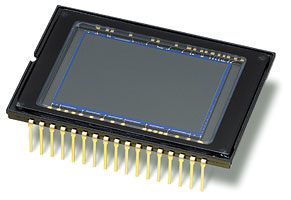
\includegraphics{immagini/ccd.png}
\caption{Un sensore CCD moderno} 
\end{figure}
Il CMOS è un sensore digitale che offre una buona qualità di immagine e costo minore,
per contro l'immagine presenta un forte rumore a causa della conversione 
analogico-digitale.\\
La visione artificiale ha tre utilizzi principali: ricognizione, identificazione, 
individuazione.
\begin{itemize}
\item \textbf{Ricognizione:} ricercare uno o più oggetti, scelti a priori, e organizzarli in 
insiemi generici o classi e mantenere informazioni riguardo il loro posizionamento 
nella scena. \\Esempio: ricercare in un'immagine o in un video tutte le persone, 
le macchine o gli animali. 
\item \textbf{Identificazione:} identificare una istanza specifica di una classe 
di oggetti. \\Esempio: ricercare in un'immagine o in un video un volto, 
una macchina o un animale specifico.. 
\item \textbf{Individuazione:} cercare una condizione specifica nell'immagine. 
\\Esempio: cercare imprefezioni nelle immagini a raggi X di superfici o materiali.
\end{itemize}
Un altro ambito in cui si sta utilizzando la visione artificiale è la modellazione
di ambienti 3D a partire da due o pià immagini 2D; questo è stato reso possibile 
grazie all'enorme aumento della capacità di elaborazione grafica delle GPU.\\
Ci sono molti altri campi in cui la visione artificiale ha rivoluzionato il settore. 
Uno di questi è la medicina dove senza questa tecnica non esisterebbero radiogradie, angiografie,
tomografie e molte altre; in questo ambito la visione artificiale salva vite identificando
anomalie e problemi come i tumori che l'occhio umano non potrebbe vedere se non 
in seguito a procedure molto invasive.
Un'altro è il controllo di veicoli autonomi, sta crescendo ad un ritmo vertiginoso
la quantità dei veicoli autonomi esistenti, sia per scopi militari sia per scopi 
civili: autovetture, droni, robot e carri per il rifornimento tutto quello che 
un tempo era naturalmente dipendente della guida umana ora può muoveri autonomamente. 
\begin{figure}[!htb] \center
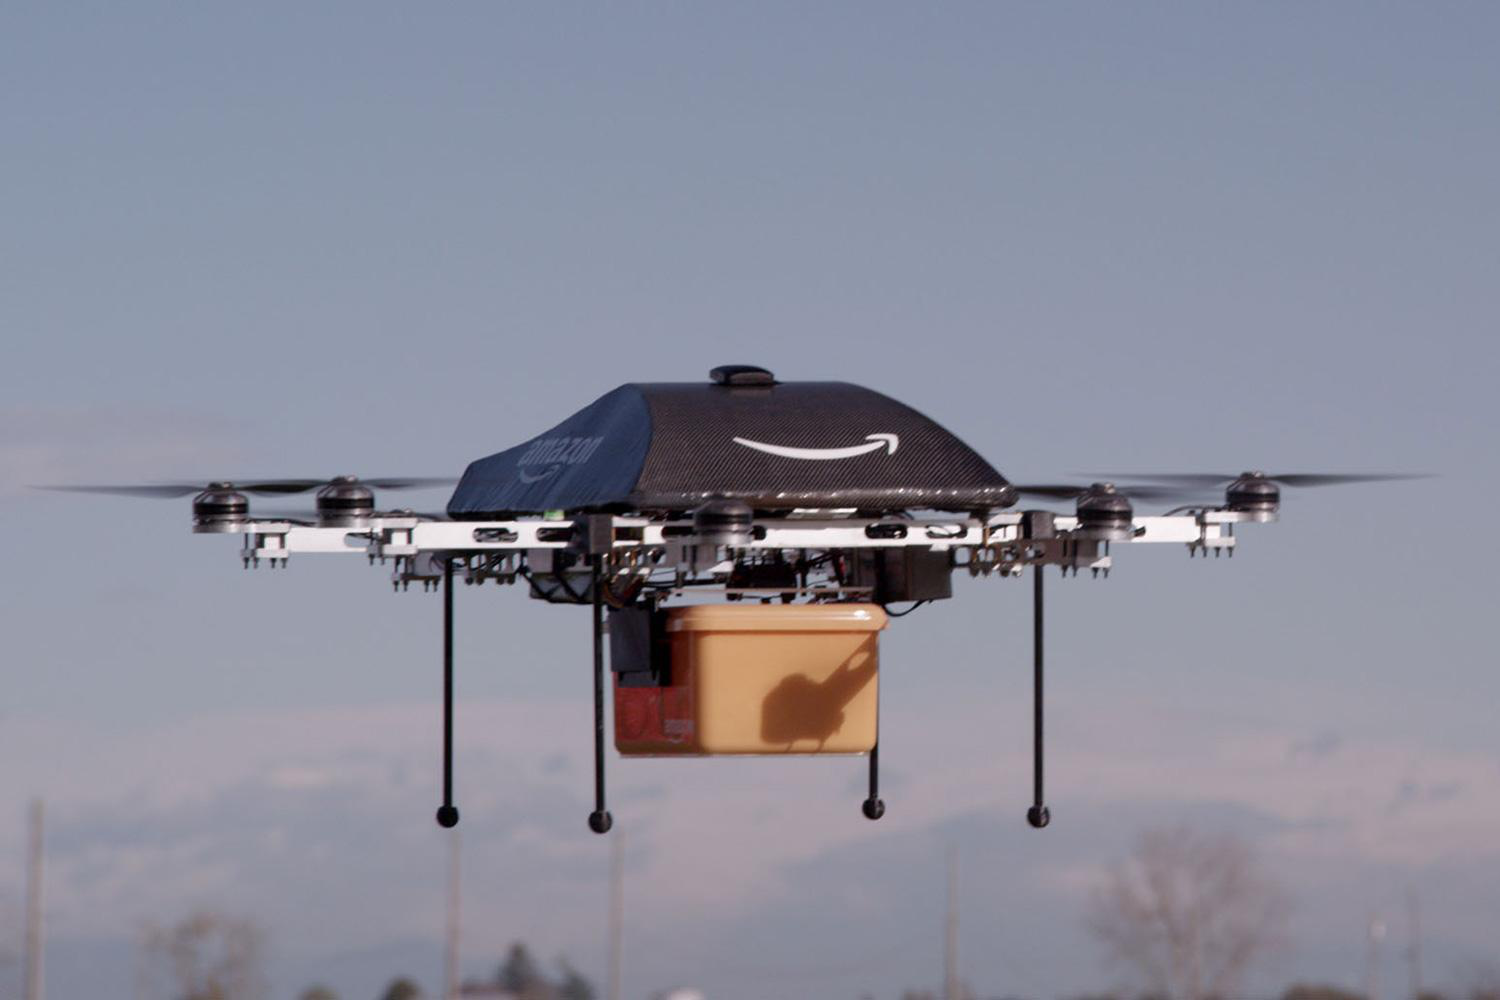
\includegraphics[scale=0.2]{immagini/amazon-air.png}
\caption{Drone della società statunitense Amazon. Consegnerà prodotti a domicilio in completa autonomia} 
\end{figure}
E' proprio in questo campo civile, o più precisamente in quello scientifico, 
che ricade il nostro lavoro di tesi su un robot autonomo per l'identificazione
di colori.

